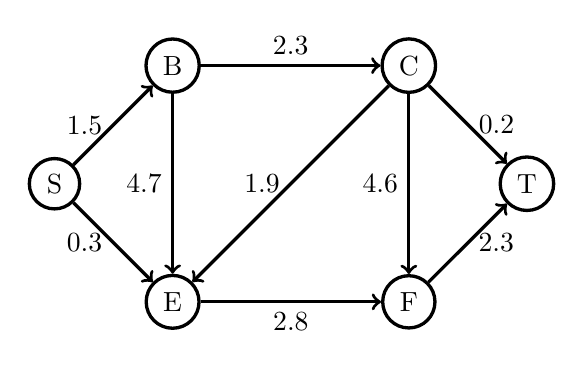
\begin{tikzpicture}[scale=0.5]
 \tikzset{directed/.style={->}} 
  \node[draw,circle, very thick] (S) at (0,3) {S};
  \node[draw,circle, very thick] (B) at (3,6) {B};
  \node[draw,circle, very thick] (C) at (9,6) {C};
  \node[draw,circle, very thick] (E) at (3,0) {E};
  \node[draw,circle, very thick] (F) at (9,0) {F};
  \node[draw,circle, very thick] (T) at (12,3) {T};
  \draw[very thick, directed] (S) -- node[left] {1.5} (B) ;
  \draw[very thick, directed] (S) -- node[left] {0.3} (E);
  \draw[very thick, directed] (B) -- node[above] {2.3} (C);
  \draw[very thick, directed] (B) -- node[left] {4.7} (E);
  \draw[very thick, directed] (C) -- node[right] {0.2} (T);
  \draw[very thick, directed] (C) -- node[left] {1.9} (E);
  \draw[very thick, directed] (C) -- node[left] {4.6} (F);
  \draw[very thick, directed] (E) -- node[below] {2.8} (F);
  \draw[very thick, directed] (F) -- node[right] {2.3} (T);
\end{tikzpicture}
